\documentclass{article}

\usepackage[english]{babel}
\usepackage[utf8]{inputenc}
\usepackage{fancyhdr} %headers and footers

\usepackage{graphicx}
\graphicspath{ {./Tensorboard_images/} } %images insertion

\usepackage{float} %tables positioning

\usepackage{flafter} %better table positioning

\usepackage{amsmath}
\pagestyle{fancy} %headers and footers declaration
\fancyhf{}
\rhead{Corda F. Franchin L.}
\lhead{Kaggle Competition}
\rfoot{\thepage}
\renewcommand{\footrulewidth}{1pt}

\title{Artificial Neural Networks \& Deep Learning Project}
\author{Team 10520637\_10527649}

\begin{document}	
	\maketitle

	\section{Convolutional Neural Network}
	
	We started from the model provided during the lab lectures to understand how the process worked.
	
	\begin{enumerate}
		\item To solve the splitting between the validation and training set we used the parameter validation\_split=0.8 in the ImageDataGenerator constructor.
		\item To adapt the test images to the input size we use the Image.resize() method.
	\end{enumerate}	
	
	\begin{figure}[H]
		\centering
			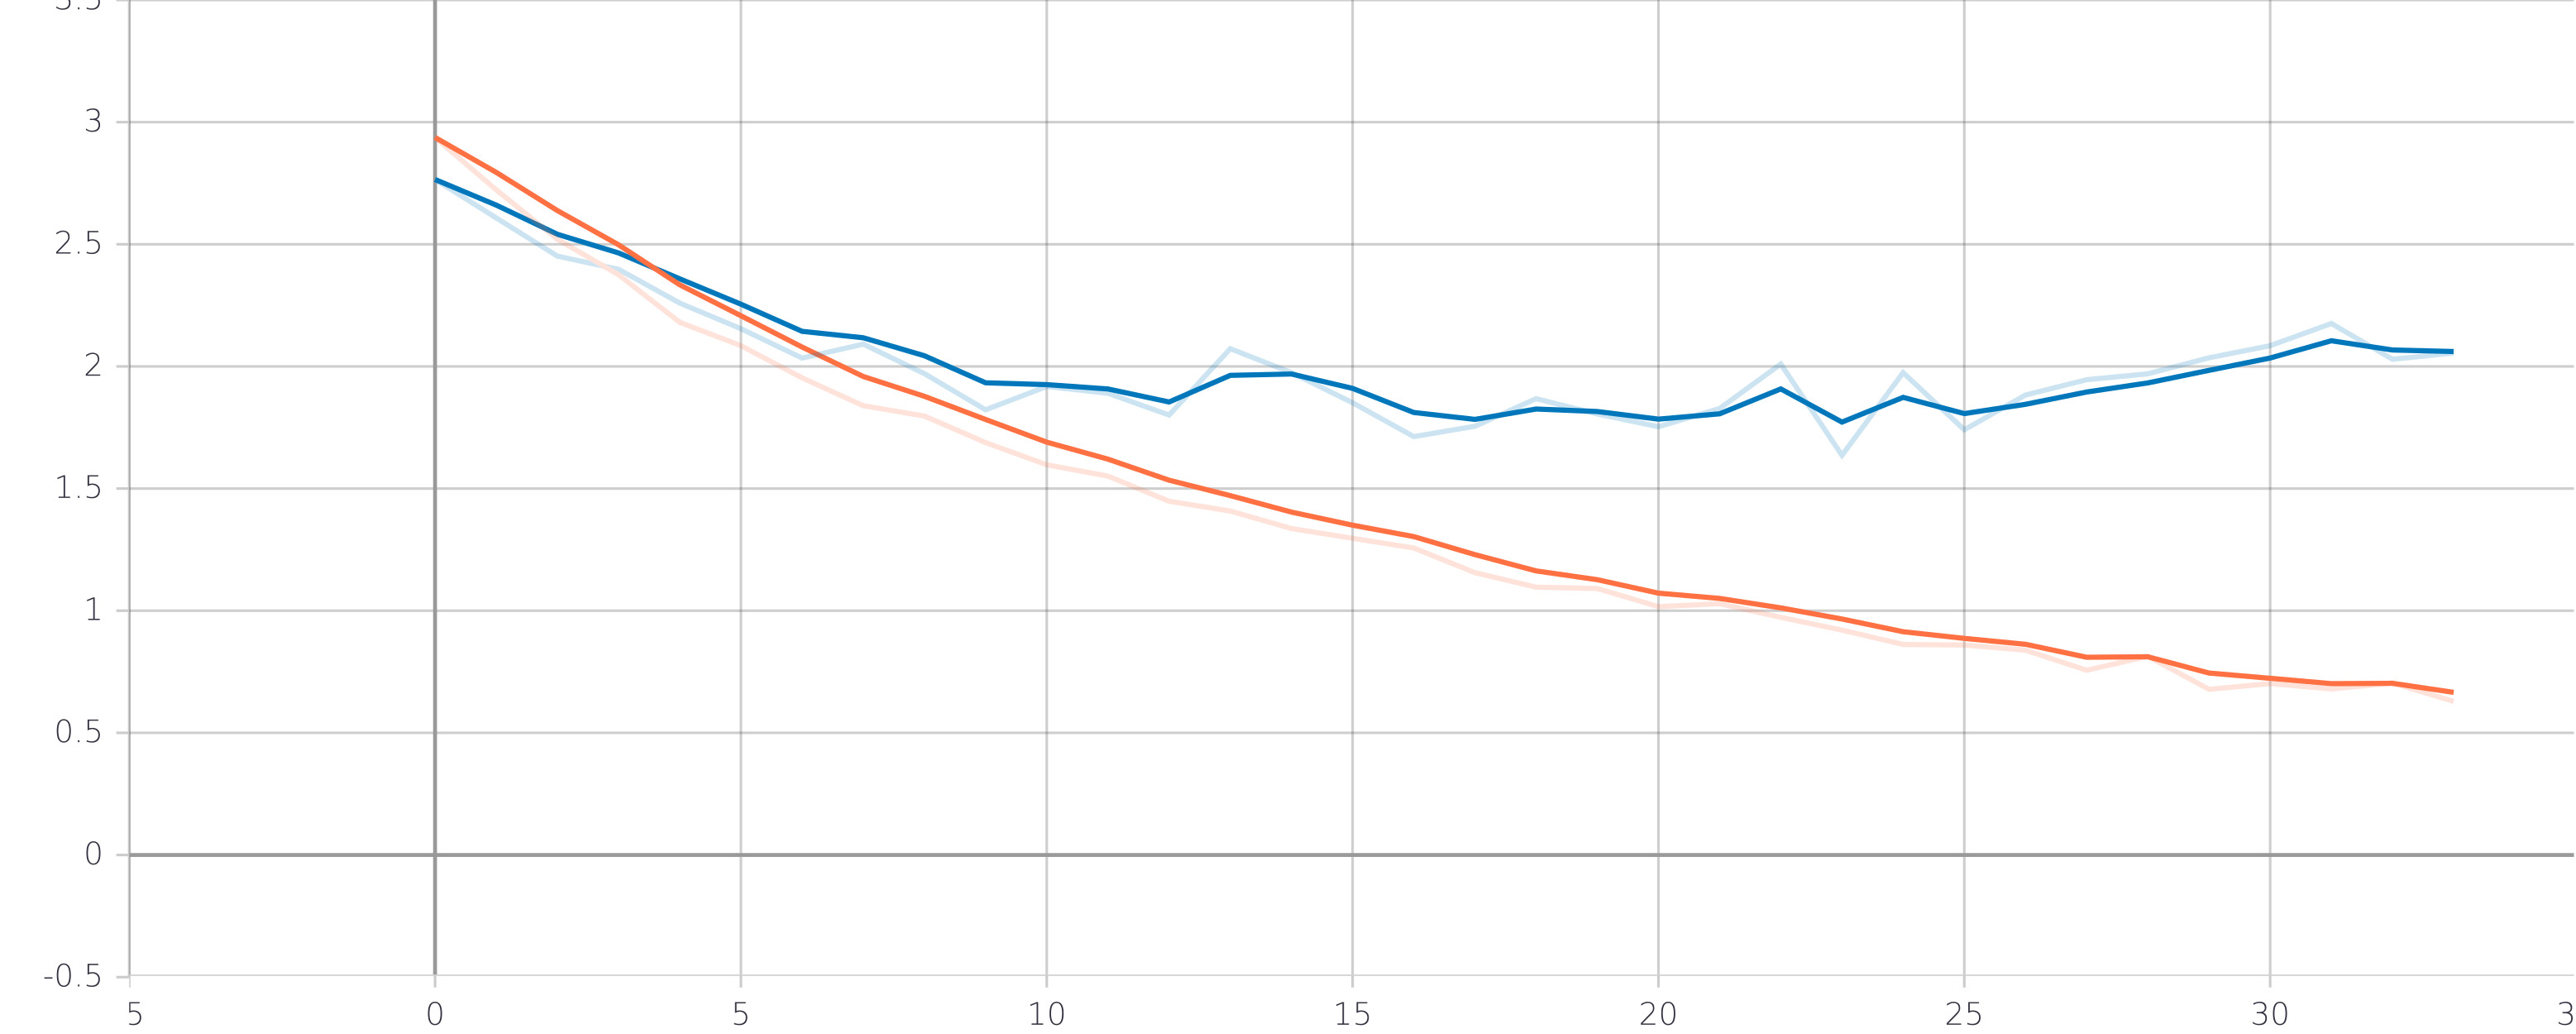
\includegraphics[width=9cm, keepaspectratio]{CNN_LOSS.jpg}
			\caption{CNN \texttt{val\_loss} plot}
	\end{figure}
	
	\begin{figure}[H]
		\centering
			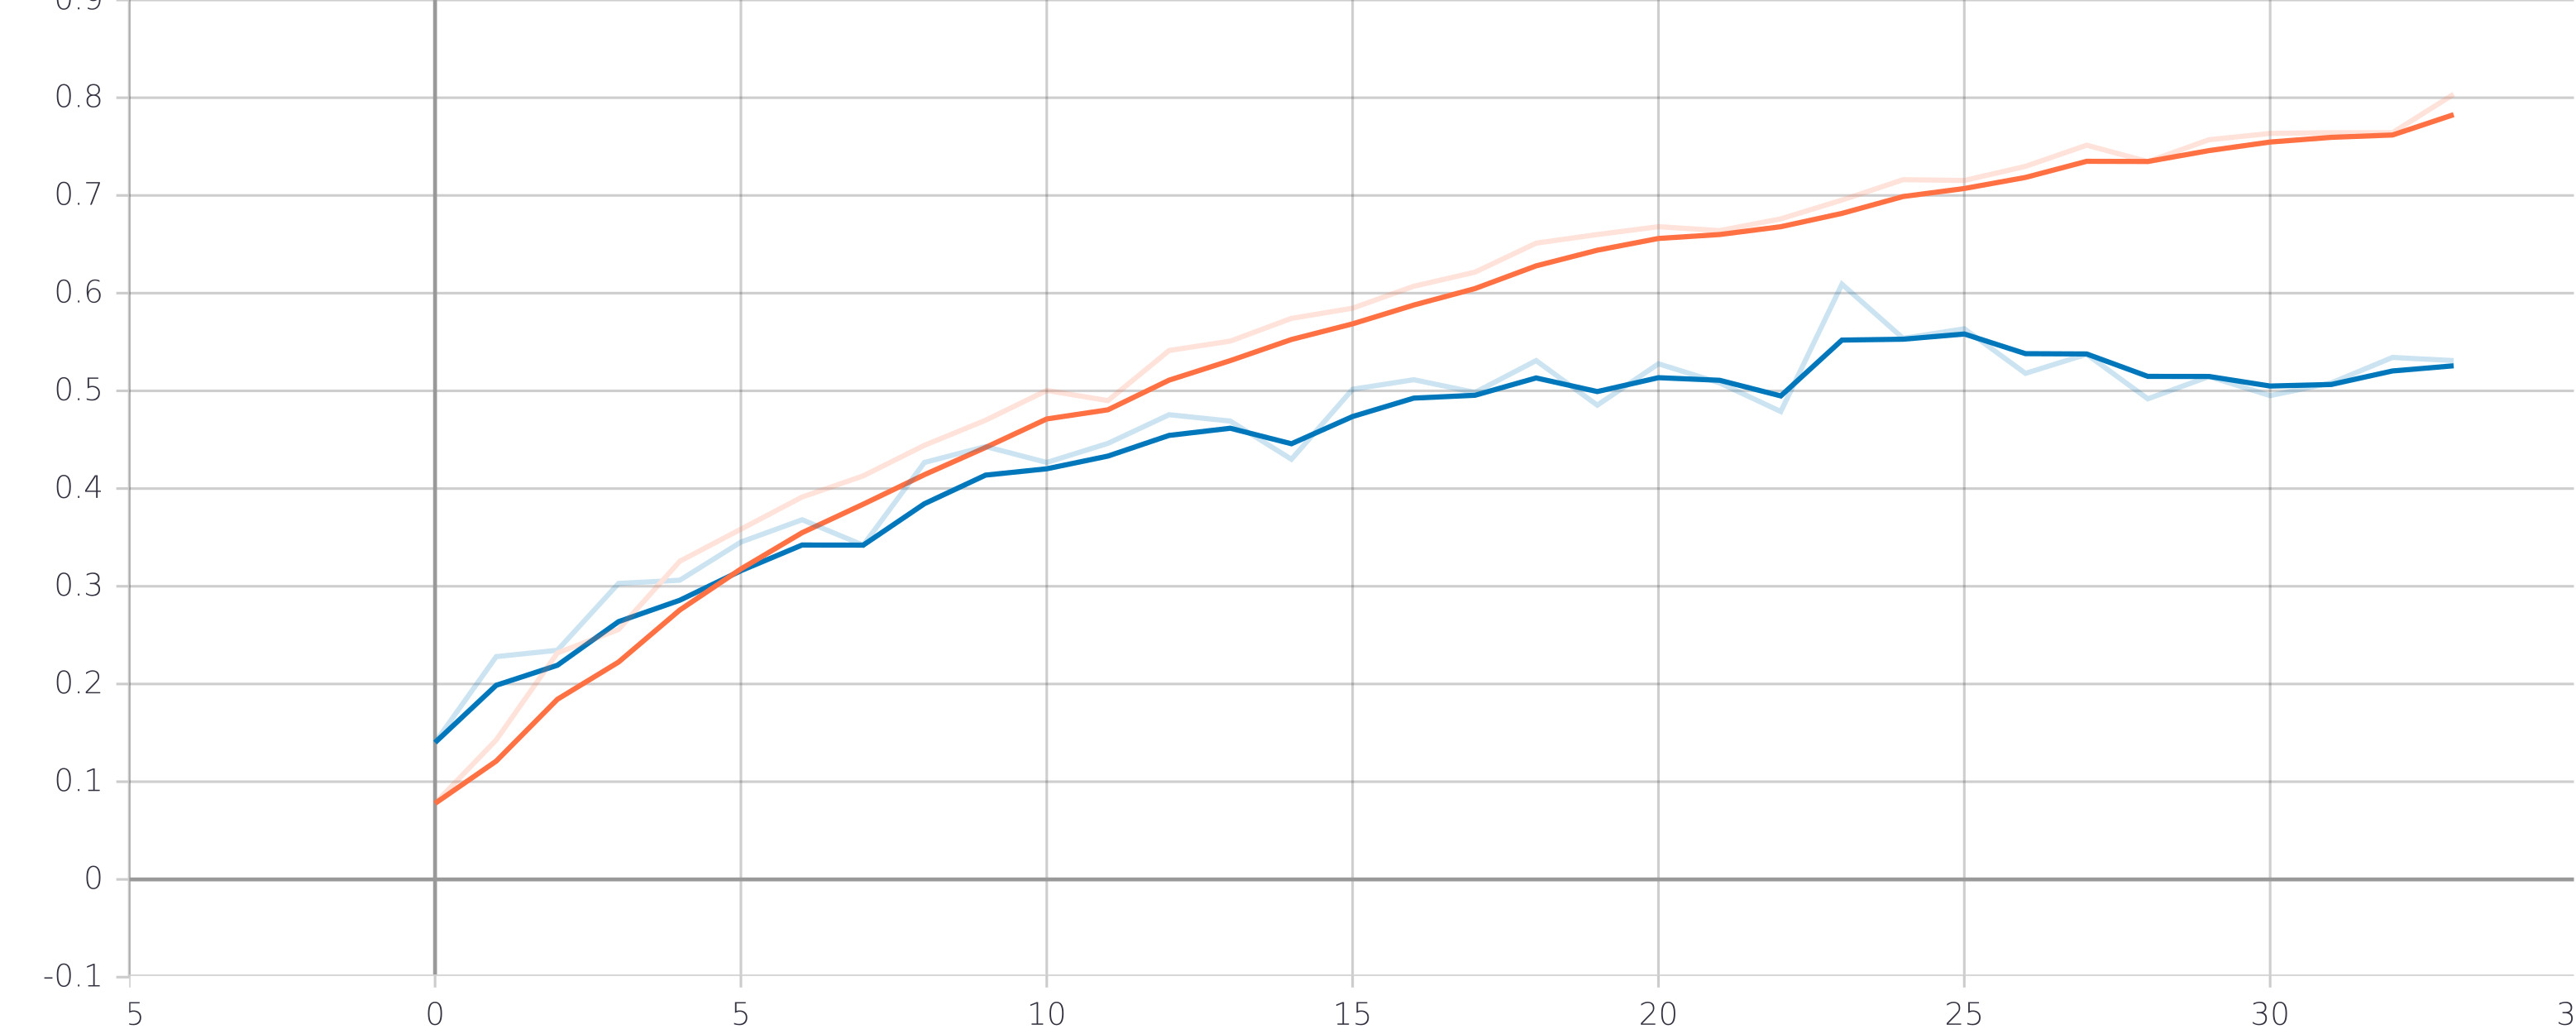
\includegraphics[width=9cm, keepaspectratio]{CNN_ACC.jpg}
			\caption{CNN \texttt{val\_acc} plot}
	\end{figure}
		
	
	\subsection{Dropout and Early Stopping}
	After our first submission we tried to change the architecture adding a dropout layer. The new model showed a slow learning rate and no particular improvements. \\
	We modified the patience and the min\_delta values of the Early Stopping callback. Increasing the patience of the callback showed us that the model stopped learning and the performance increases were very little.
	
	\subsection{Network Depth}
	We tried to add some convolutional layers to the network by simply changing the depth parameter, after some epochs in which the network didn't learn we understood that the receptive field was too high and the max-pool layers should be reduced. \\
	We tried to modify the convolutional block itself by doubling the convolutional layers in each block.\\
	We tried to completely modify the network structure by building sequentially the architecture, consisting of 2 blocks of 2 convolutional layers  and 3 blocks of 3 convolutional layers. \\
	We tried to modify the classifier by adding two layers resulting in a network with \(512 \rightarrow 256 \rightarrow 128\) neurons.

	\newpage
	
	
	We repeated the experiment with a network with \(512 \rightarrow 512 \rightarrow 256\) neurons.\\
	After all these tries the validation accuracy did not increase.
	
	\section{Transfer Learning: VGG16}
		We firstly tried with the code provided during the laboratory session and set the freeze value to 18 thus training only the last 5 layers plus the classifier itself. This turned out in huge performance improvement. \\
		\texttt{train\_acc=0.9126} \\
		\texttt{val\_acc=0.6808}
		
		\begin{figure}[H]
			\centering
			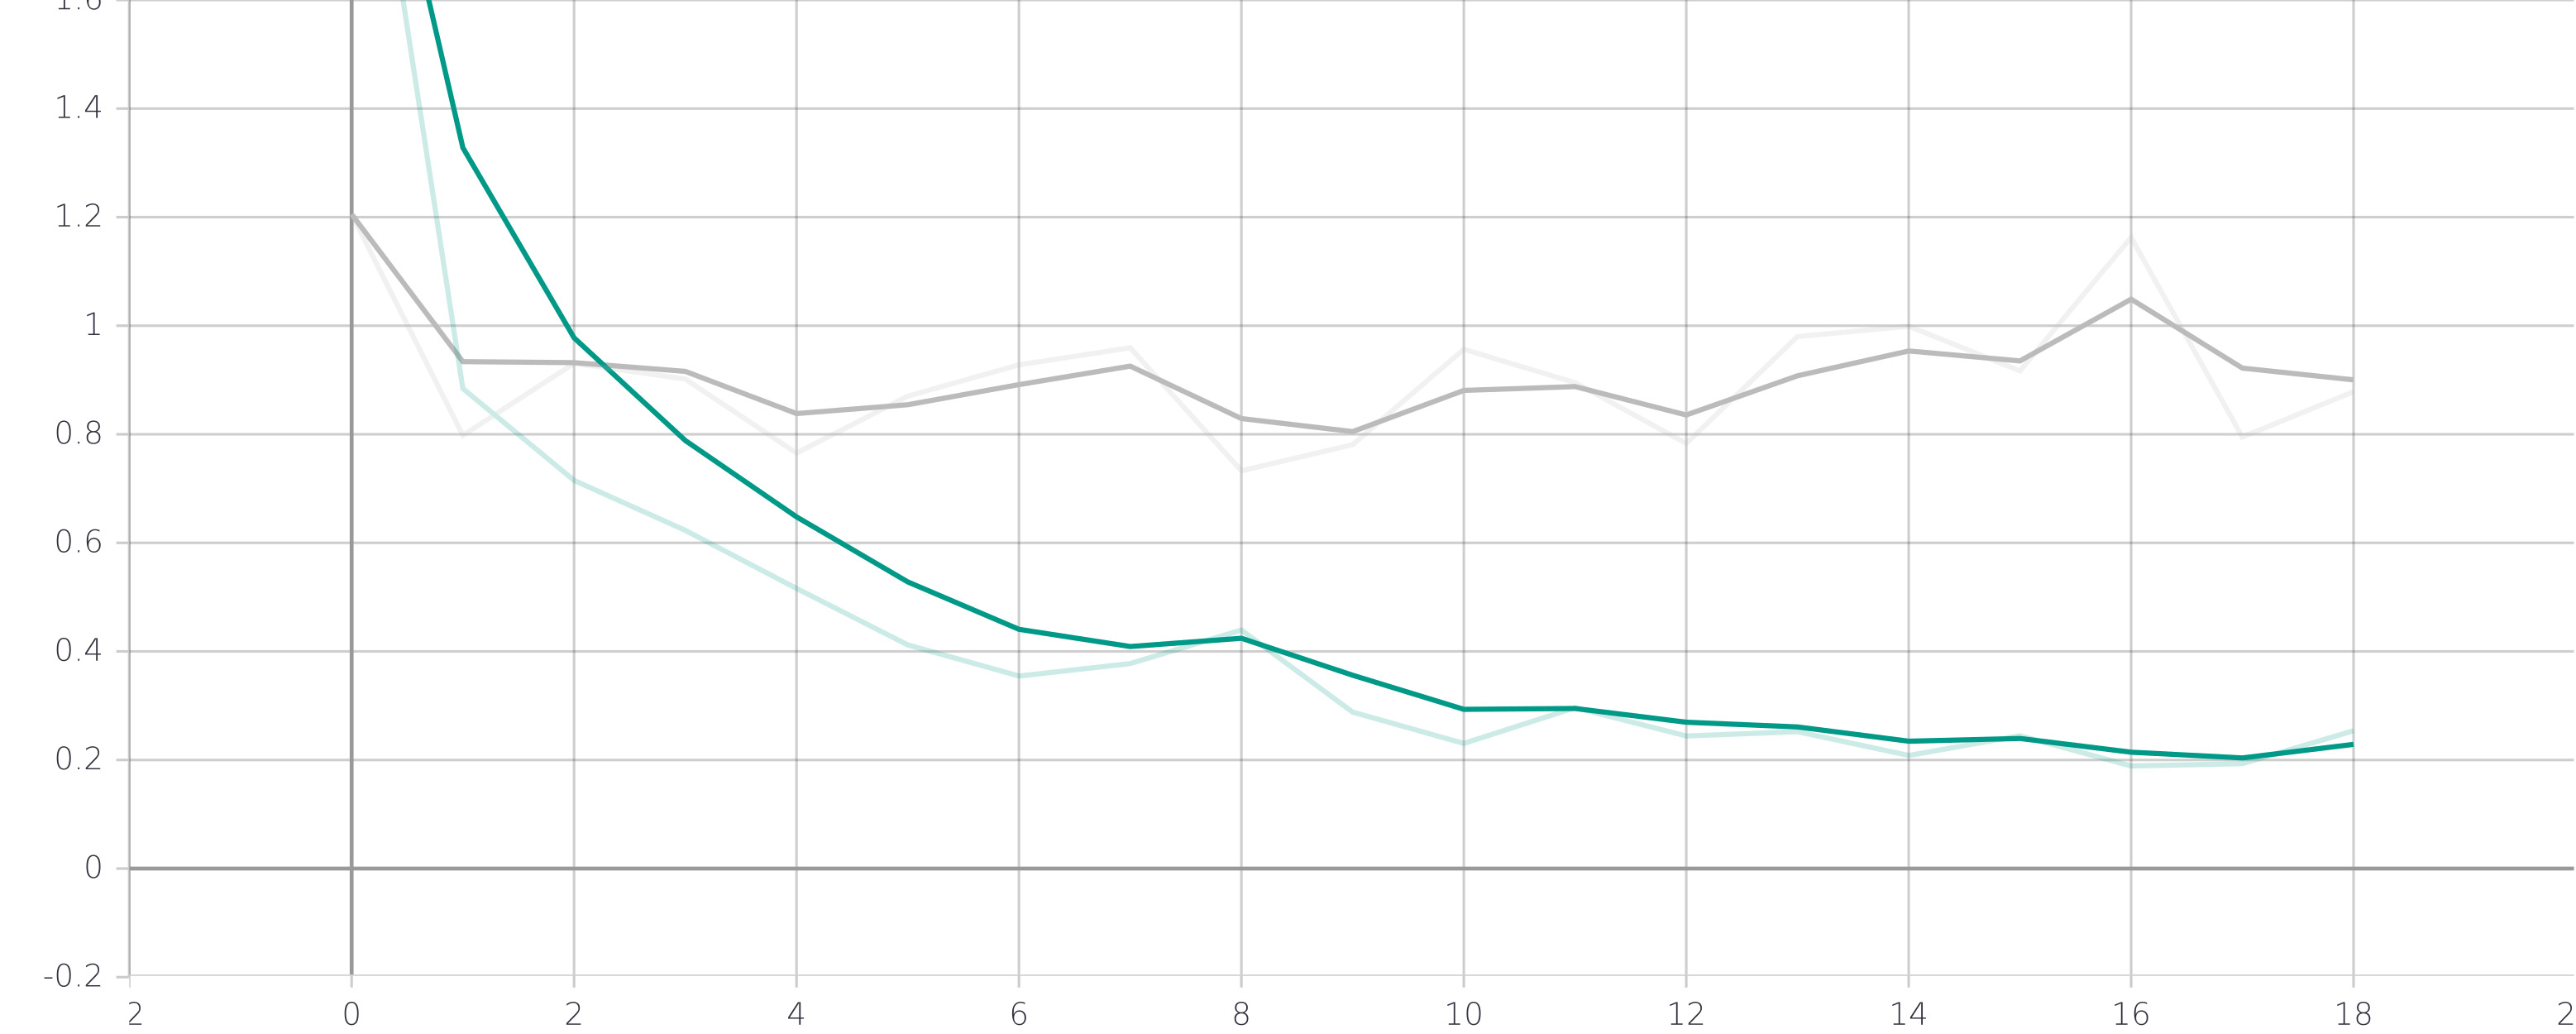
\includegraphics[width=9cm, keepaspectratio]{VGG_LOSS.jpg}
			\caption{VGG16 \texttt{val\_loss} plot}
		\end{figure}
	
		\begin{figure}[H]
			\centering
			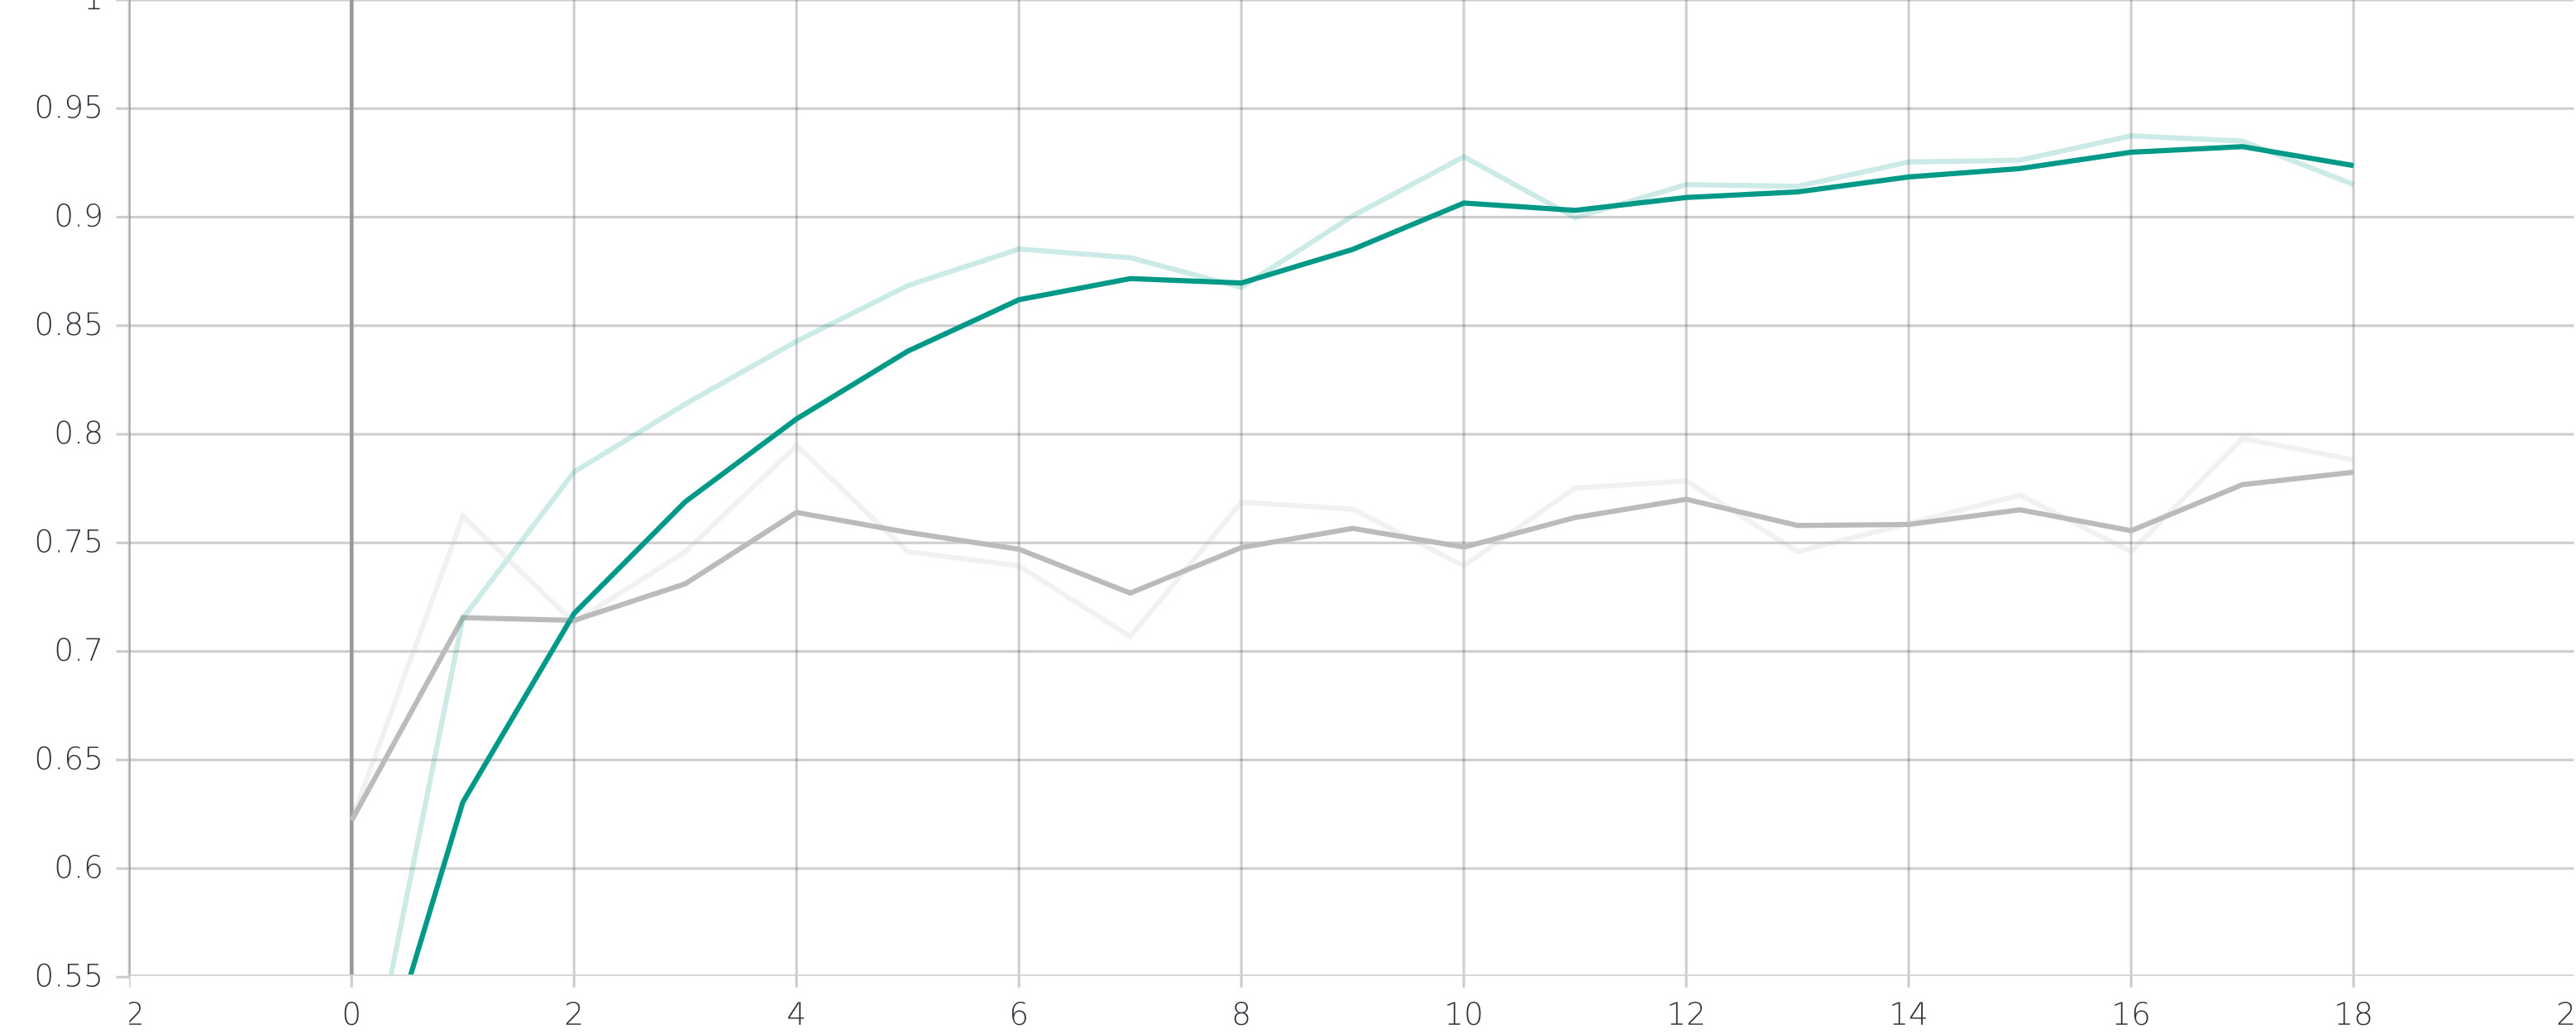
\includegraphics[width=9cm, keepaspectratio]{VGG_ACC.jpg}
			\caption{VGG16 \texttt{val\_acc} plot}
		\end{figure}
		
		\subsection{Data Augmentation Correction}
			Through the development of our project, we observed that applying data augmentation to the validation set could turn out in a pessimistic evaluation of the model performances. Instead of using the internal function of DataImageGenerator we implemented an algorithm to split the training set into two separate folders and then apply data augmentation only on the training dataset. This resulted in a more accurate validation score concerning the test performance.
			
	\section{Transfer Learning: Xception}
		Considering all the available architectures saw during lectures VGG16 looked too heavy and not so performing. We applied Transfer Learning with Xception architecture without fine-tuning, we trained only the classifier. This showed immediate performance improvements.
		
		\begin{figure}[H]
			\centering
			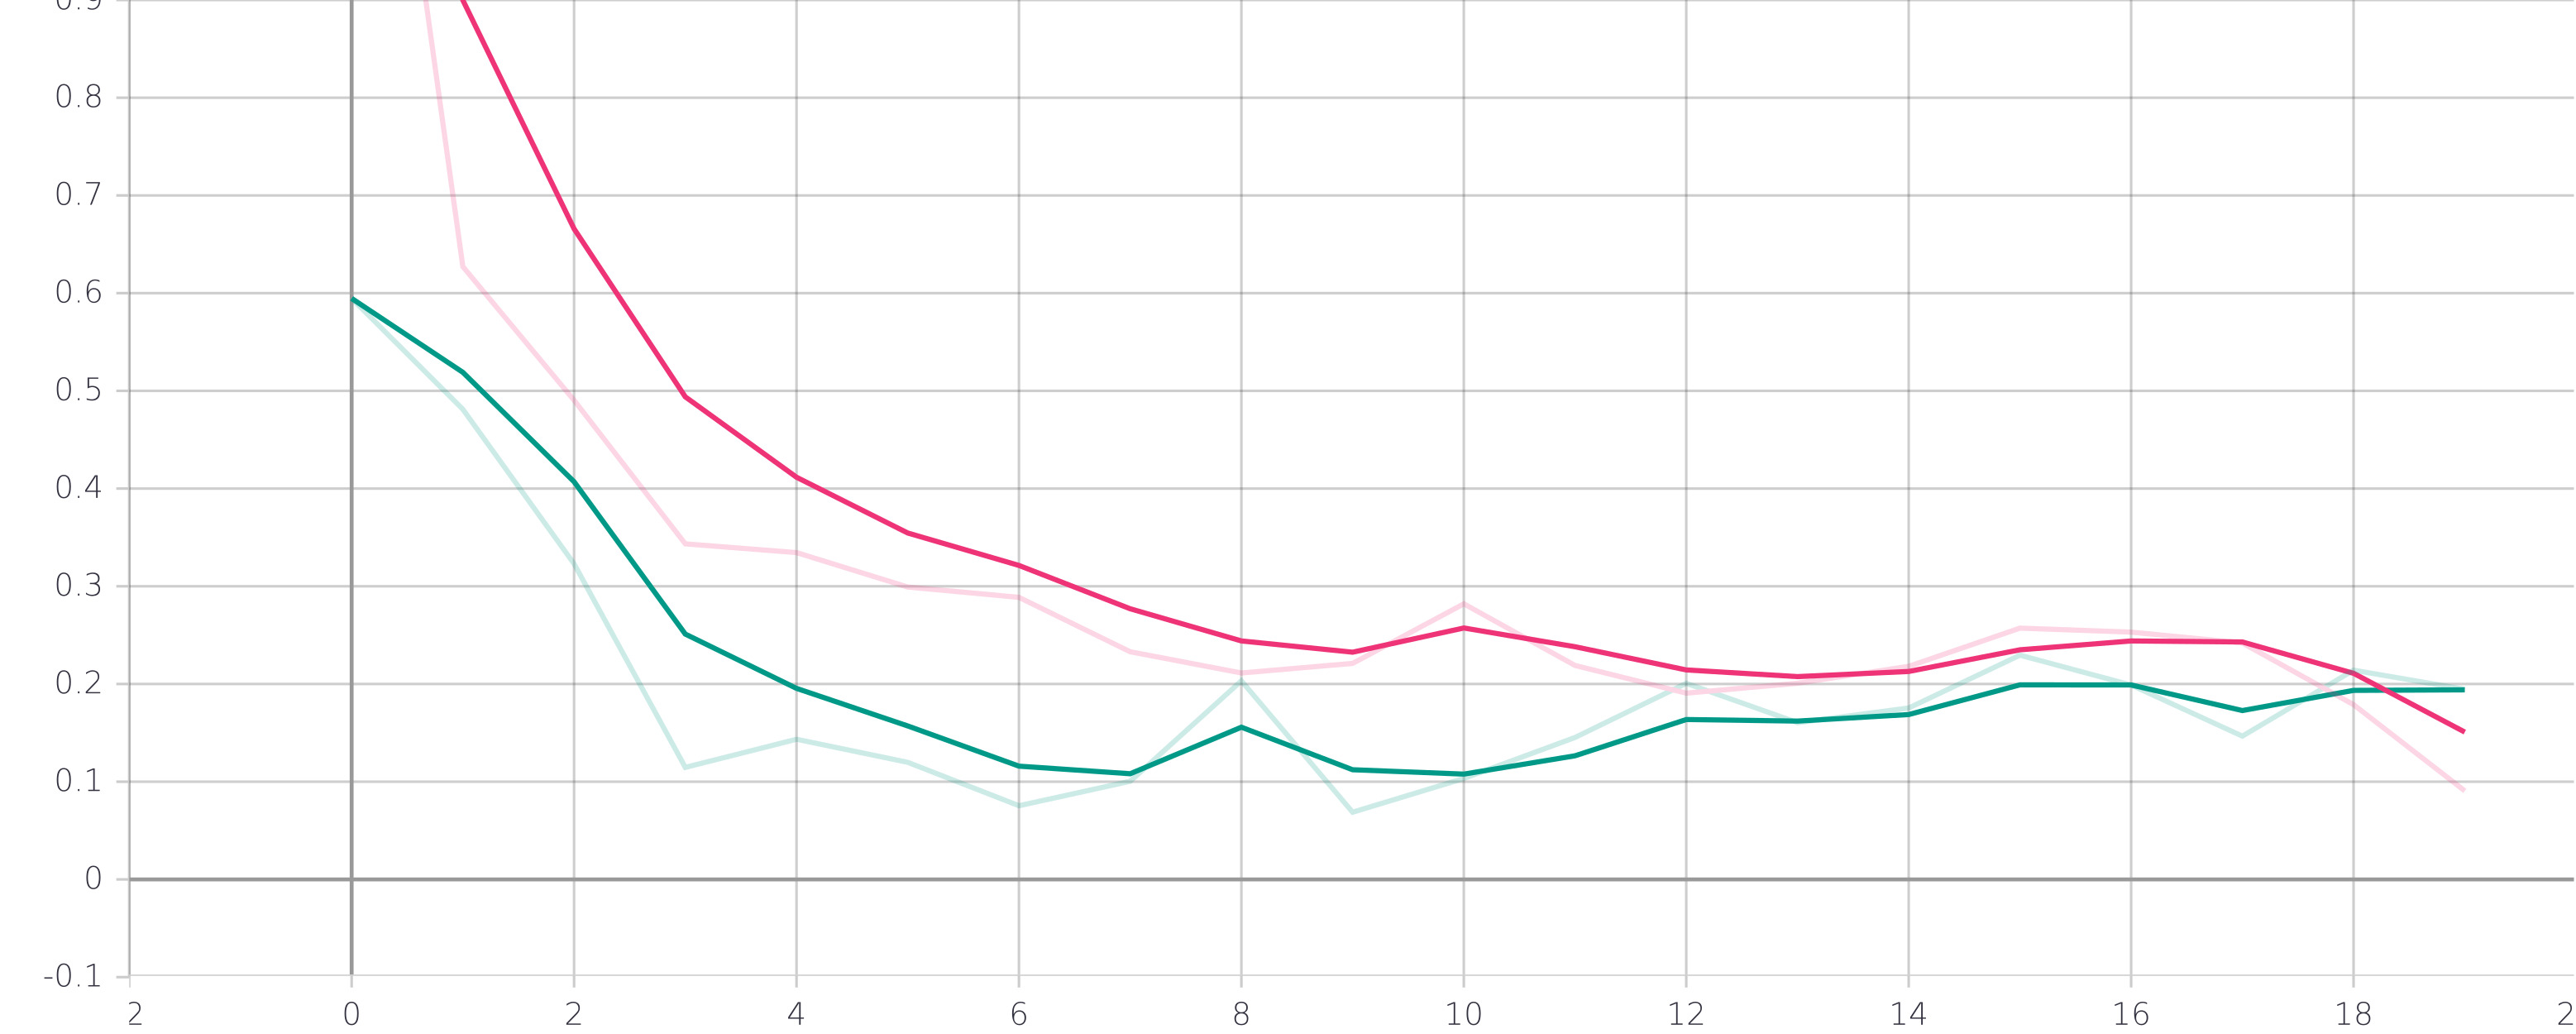
\includegraphics[width=9cm, keepaspectratio]{XCEPTION_LOSS.jpg}
			\caption{XCEPTION \texttt{val\_loss} plot}
		\end{figure}
	
		\begin{figure}[H]
			\centering
			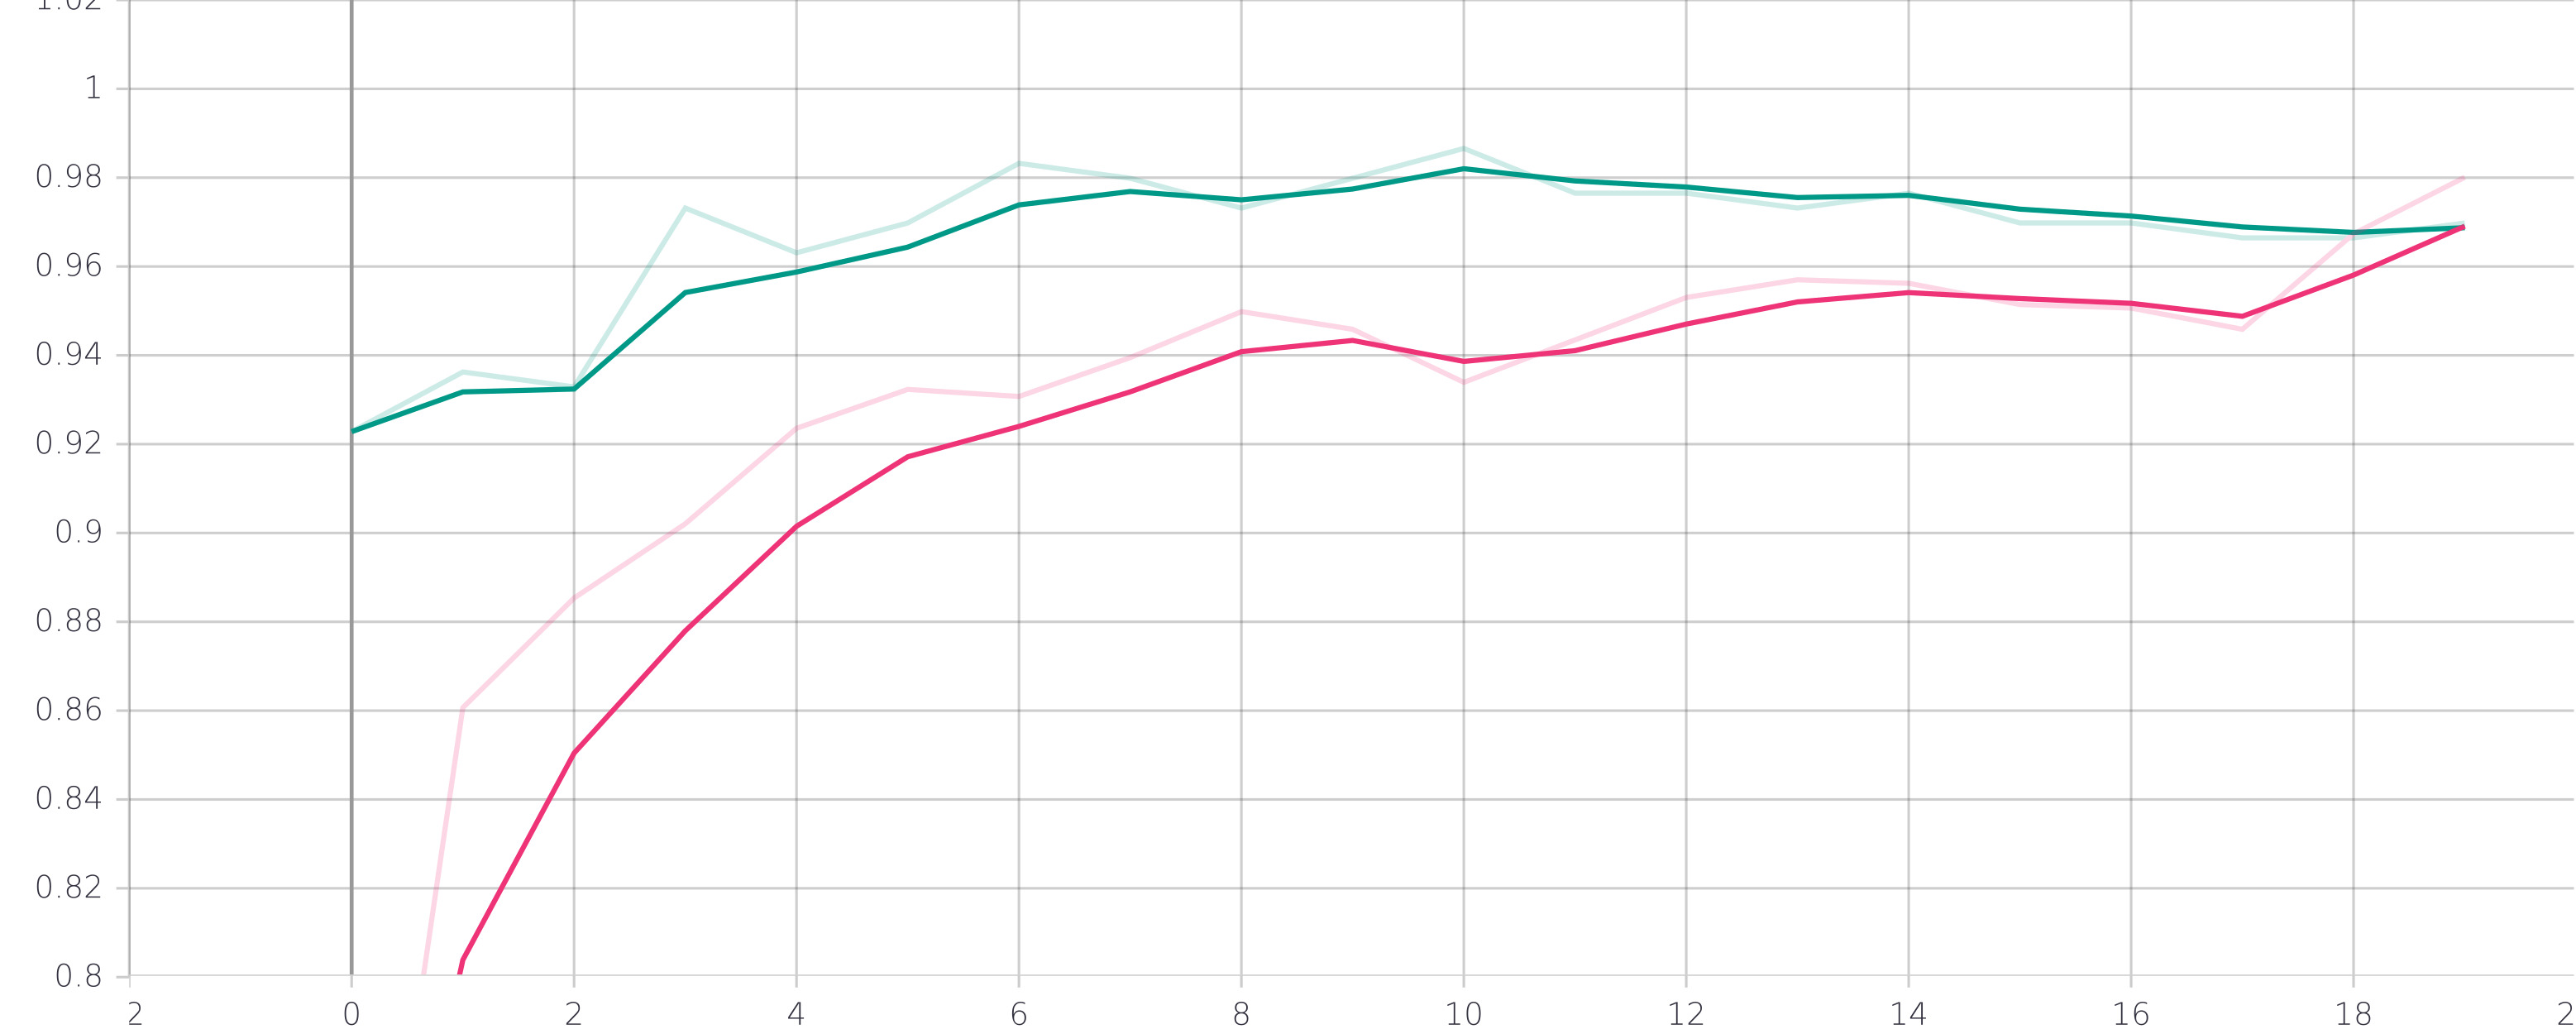
\includegraphics[width=9cm, keepaspectratio]{XCEPTION_ACC.jpg}
			\caption{XCEPTION \texttt{val\_acc} plot}
		\end{figure}
		
		\subsection{Fine Tuning}
		
			\begin{enumerate}
				\item We started training only the classifier with a specific dataset split.
				\item We shuffled again the dataset, changing the validation split. Then we trained the network unfreezing the weights of the last 6 layers of Xception.
			\end{enumerate}
			
			\noindent
			
			This showed a small improvement in validation accuracy.		
			
		\subsection{Global Average Pooling \& Max Pooling} 
			
			We tried to add a Global Average Pooling layer at the end of the network and restart the process of fine-tuning. Then we repeated this process with Global Max Pooling. The best results were found with the second architecture. 
		
\end{document}